\documentclass[a4paper,12pt,twoside,openright]{report}

\usepackage{graphicx}
\usepackage[pdfauthor={George Boyle},%
pdftitle={A Scheme To Lua Translator},%
pagebackref=true,urlcolor=blue,%
colorlinks,pdftex]{hyperref}
\usepackage{verbatim} % TODO Remove this

\linespread{1.2}


\begin{document}


\begin{comment} % TODO Remove this
\title{A Scheme To Lua Translator \\
{\small 4th Year Computer Science Project} \\
{\small University College Cork}}
\author{Student: George Boyle \\ Student Number: 106827004 \\ \\
Supervisor: Dr.\ Joseph Manning \\
Second Reader: Prof.\ Gregory Provan}


%
% Title Page, Abstract & Table Of Contents
%

\maketitle
\begin{abstract}
Scheme and Lua are two neat programming languages that have many similarities
and many differences. This project is an exploration of the relationship between
them. It takes the form of a one-way source-to-source translator from Scheme to
Lua, aimed at uncovering the gamut of expressibility, and finding insights into
the essence of computer languages. \\[10mm]

\begin{center}\textbf{Declaration Of Originality}\end{center}

\noindent I hereby declare that:
\begin{itemize}
\item this is all my own work, unless clearly indicated otherwise, with full and
proper accreditation;
\item with respect to my own work: none of it has been submitted at any
educational institution contributing in any way towards an educational award;
\item with respect to another's work: all text, diagrams, code, or ideas,
whether verbatim, paraphrased or otherwise modified or adapted, have been duly
attributed to the source in a scholarly manner, whether from books, papers,
lecture notes or any other student's work, whether published or unpublished,
electronically or in print.\\[5mm] 
\end{itemize}
\begin{tabular}{rl}
\textbf{Name:} & George Boyle \\[8mm]
\textbf{Signed:} & \rule[-0.4mm]{5cm}{0.4pt} \\[8mm]
\textbf{Date:} & \today
\end{tabular}

\end{abstract}

\tableofcontents


%
% Main Document
%

\chapter{Background (10 pages)}
\section{Introduction (4 pages)}
Blah blah blah

\section{About Scheme (3 pages)}
Blah blah blah

\section{About Lua (3 pages)}
Blah Blah Blah


\chapter{Project Administration (5 pages)}
Project development took place from late November 2009 to late March 2010. As
the period progressed, there was a cumulative increasing focus on the project
work, as the workload from other assignments receded. Work was characterised by
regular meetings with the supervisor, with a number of periodic code
submissions.

Given that this was a reasonably small, single-person project, and somewhat
experimental in nature, formal project management methodologies were not
rigorously applied. Instead it was managed through constant attention, with the
help of some software tools.


\section{Methodology}

The project followed a mainly evolutionary lifecycle. It was also clear from the
beginning that it would not be possible to have a thoroughly complete translator
in the available time.  As a result, the project followed the course of a
prioritised list of objectives, which were followed in a serial fashion for the
most part.  Certain minor features were worked on in parallel, and the source
code management system facilitated that, but this was largely the exception for
two reasons: firstly each feature needed to be completed in full to avoid
breaking the entire program; and secondly, there was significant linear
dependency between features.


\section{Supervisor Meetings}

The supervisor meetings were held in Dr.\ Manning's office on a weekly basis,
usually on Thursday afternoons. The meetings generally had the following format:

\begin{enumerate}
\item An investigation of some specific problems encountered
\item A general discussion of the current state of the project, of the
features of Scheme and Lua, and the similarities and differences between
them
\item A look at the project direction and goals in high-level terms
\end{enumerate}

The frequency of the meetings helped the momentum of the project, and it meant
that potential pitfalls could be confronted and dealt with on a regular basis.
Revisiting and revising objectives every week made it flexibile and dynamic,
which facilitated exploration of specific areas when necessary.


\section{Tools}

\subsection{Text Editor}

The \emph{vim}\footnote{\url{http://www.vim.org}} editor was used to create and
edit all of the source code. Vim stands for Vi-Improved, a feature-rich version
of the old UNIX editor. It is widely available, versatile and highly
configurable. Among other things, it contains automatic indenting and syntax
highlighting making it more than adequate for a project such as this. In any
case, the volume of code didn't warrant a large Integrated Development
Environment.

\subsection{Version Control}

It was decided that the project source code should be managed using
VCS\footnote{Version Control System} software, rather than do it manually. This
had numerous advantages, including keeping a record of the project's history,
data backup and synchronisation across computers. A number of tools were
considered. One was
\emph{Subversion}\footnote{\url{http://subversion.apache.org/}}, a centralised
version control system. This was a natural choice as it is available on the lab
computers, and there is an svn repository running on \emph{cosmos.ucc.ie}.
However, the flood of November 2009 and its effect on the availability of
\emph{cosmos} meant that an alternative needed to be found.

This presented a great opportunity to try a modern distributed version control
system. The distributed model made more sense, particularly in this context, for
the following reasons:

\begin{description}
\item[Availability] \hfill \\
As mentioned above, the primary motivator for the move was the availability of
\emph{cosmos}, as it regularly had to be taken offline to service the generators
in the wake of the flood. 
\item[Data Backup] \hfill \\
Without a central server, there is no ``single point of failure''. Backing
up the entire history became simply a matter of working on the project from a
number of different computers. It was also possible to regularly synchronise
with an online code repository, for further redundancy.
\item[Workflows] \hfill \\
The range of possible workflows for a distributed VCS is greater than for a
centralised one. Being a single-person project, the centralised model is
unnecessary and prohibitively restrictive.
\item[Speed] \hfill \\
A distributed VCS doesn't suffer the network latency overheads of a centralised
system for the majority of its operations. Though this is not hugely significant
for such a small project, over time the delay adds up, so it was still a
consideration.
\item[Relevance] \hfill \\
There is an increasing trend in free and open-source projects towards
distributed version control, so this presented a chance to acquire skill in an
important contemporary tool.
\end{description}

The first one to be used was
\emph{Bazaar}\footnote{\url{http://bazaar-vcs.org/}}, which is closely
associated with Canonical Ltd.\ and the Ubuntu operating system. It has some
commands in common with Subversion, making it easy to make the move. It was used
to track the project for a period from November to January, but it proved to be
a bit slow, and there was some difficulty getting it to work through the
University firewall.

At the beginning of February, the project was moved to
\emph{Git}\footnote{\url{http://git-scm.com/}}. Git is another open source
distributed version control system, developed by Linus Torvalds in 2005 to track
the source code of the Linux kernel, replacing the proprietary \emph{Bitkeeper}
system. It is more difficult to learn, but it is very neat in concept, and is
considerably faster than Bazaar for normal use.

The online Git repository for this project, which includes the project history
since 1st~February~2010, can be found at:
\begin{center}\url{http://github.com/Dockheas23/scheme2lua}\end{center}

\subsection{Typesetter}

This report was written and typeset using
\LaTeX\footnote{\url{http://www.latex-project.org/}}, with support for
generating pdf files. It was originally created by Leslie Lamport as a
convenient and usable set of macros for Donald Knuth's typesetting system, \TeX.
It has become a de-facto standard for scientific papers, and produces
well-structured and aesthetically pleasing documents.

\subsection{Graphics, Diagrams \& Presentation}

\emph{OpenOffice}\footnote{\url{http://www.openoffice.org/}} is a complete open
source office suite created by Sun Microsystems.  It can work with several
formats, including the standard OpenDocument format as well as Microsoft's
proprietary file formats. Its drawing and presentation programs were used to
create the diagrams and slides for the project open day.

Another open source program called
\emph{Dia}\footnote{\url{http://projects.gnome.org/dia/}} was used to create the
UML diagrams in later sections of this report. It is part of the
\emph{GNOME}\footnote{\url{http://www.gnome.org/}} project and can work with a
variety of different types of flow-charts and block diagrams, using a simple
drag-and-drop interface. It also contains an automatic code generation function,
and can export to a number of file formats, including png, pdf, eps and svg.


\chapter{The Translator}
Here goes an introduction to this chapter and the sections to come.


\section{Requirements}

Being a project that is experimental and research-oriented in style, the
requirements could not be rigidly determined in fine detail at the outset, or
even at later stages. However it was certainly possible, and indeed important,
to establish a set of high-level requirements and guiding principles for the
project. These were categorised as functional and non-functional requirements.

\subsection{Functional Requirements}

\begin{itemize}
\item The program must take a Scheme program as input and output a Lua program
as output
\item When the Lua output from the program is run through a Lua interpreter, it
must produce the same output as the Scheme program run natively through a Scheme
interpreter.
\end{itemize}

\subsection{Non-functional Requirements}

\begin{itemize}
\item The running time of the resulting Lua program should be as short as
possible
\item The output of the program should be readable Lua code as much as possible
\end{itemize}

In particular, the non-functional requirements, though in conflict with each
other to a certain extent, pointed to simplicity as a primary design objective.


\section{Design And Implementation}

\subsection{First Approach}

The initial approach involved finding for each construct in Scheme, its most
precise and efficient representation in Lua. In French parlance, this is nicely
described by the phrase ``le mot juste'', meaning ``the precise word'' or ``the
perfect word'', and it brings to mind the image of an expert translator of
human languages, who knows through experience how to accurately convey the
intended semantic of each phrase from one language to another for a particular
context.  At first, this seemed like a reasonable and credible way of
proceeding given the small size of the core of the Scheme language.

However it soon became apparent that this approach would quickly become
unwieldy, as the range of various contexts in which an expression could appear
often meant the optimal translation needed to be adjusted slightly. An example
of this is\ldots

\subsection{Second Approach}

\begin{figure}
\centering
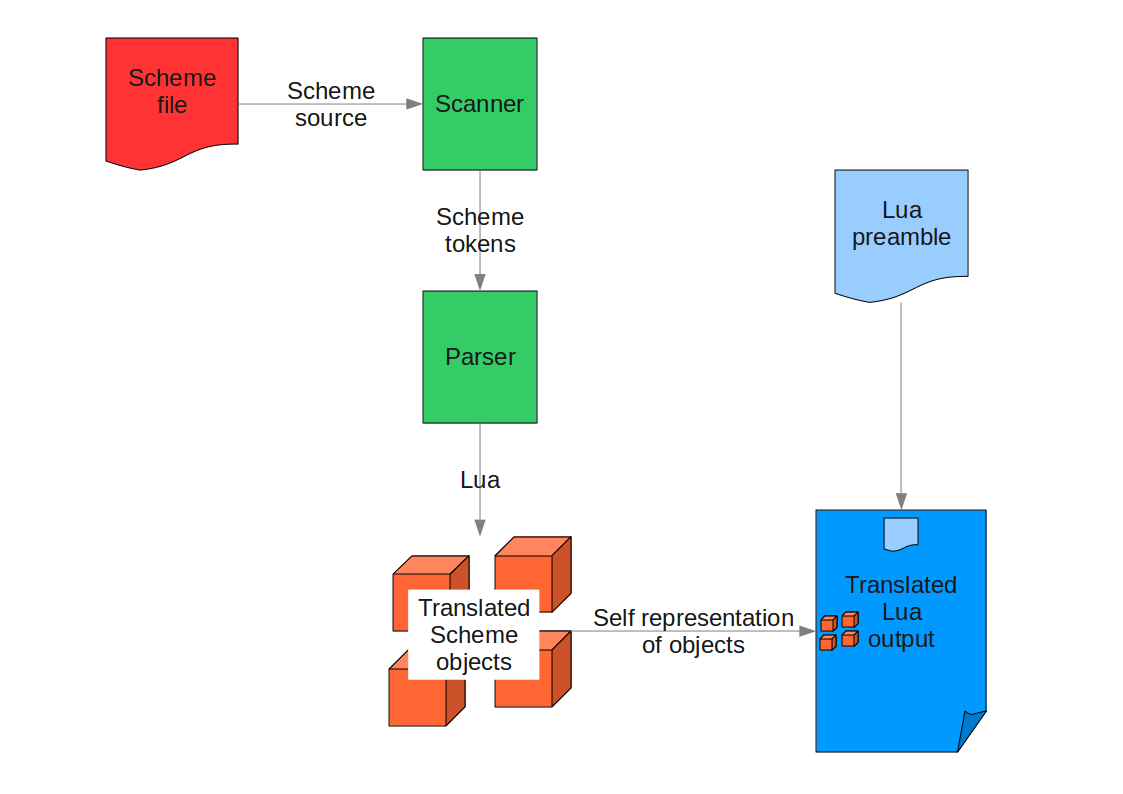
\includegraphics[width=\textwidth]{overview.png}
\caption{Overall structure of the translator}
\label{fig:overview}
\end{figure}

This approach was more structured in its implementation.


\section{Features}

\subsection{Data Types}

\begin{itemize}
\item Atomic Data
\begin{itemize}
\item Booleans
\item Numbers
\item Characters
\item Strings
\end{itemize}
\item Compound Data
\begin{itemize}
\item Lists
\item Vectors
\item Bytevectors
\end{itemize}
\end{itemize}

We will look at each of these in turn to identify what commonalities or
differences between Scheme and Lua could affect the translation.

\subsubsection{Booleans}

Being a very simple data type and having only two possible values, booleans are
easily translated. In Lua, the values are \texttt{true} and \texttt{false},
corresponding to \texttt{\#t} and \texttt{\#f} respectively in Scheme.

\subsubsection{Numbers}

Scheme has a very rich syntax for describing numbers. This is in contrast with
Lua, in which the double precision floating point number is the only
numeric type~\cite[p.10]{luabook}.

\subsubsection{Strings}

Scheme strings are more restrictive than Lua strings. ''Lua is
eight-bit clean and its strings may contain characters with any numeric code,
including embedded zeros. This means that you can store any binary data into a
string''~\cite[p.11]{luabook}.

\subsubsection{Lists}

Lists are the primary data type in Scheme, and there is a duality in the
representation of list data and the core syntax of a Scheme program.

\subsubsection{Vectors}

Vectors are similar to lists.

\subsubsection{Bytevectors}

Bytevectors are like vectors with every item representing a byte.

\subsection{Branching}

Scheme has a number of constructs for branching.

\subsection{Looping}

Including tail recursion

\subsection{Continuations}

One shot continuations using coroutines

\subsection{Syntax Extension}

syntax-rules etc.


\section{Components}

\subsection{Main Program}

Consists of a shell script that calls the main scheme2lua.lua program, which
contains the main loop.

\subsection{The Scanner}

\begin{figure}
\centering
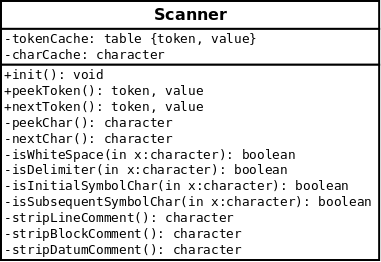
\includegraphics[width=\textwidth]{scannerUML.png}
\caption{A UML class diagram of the scanner component}
\label{fig:scannerUML}
\end{figure}

Figure~\ref{fig:scannerUML} shows the structure of the scanner in UML class
diagram form. Though it used a slightly different implementation, it was created
borrowing heavily from the ideas and techniques used in the SAL
interpreter~\cite{sal}

\subsection{The Parser}

\begin{figure}
\centering
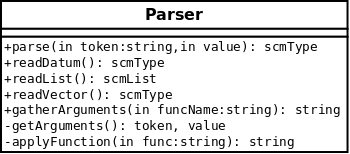
\includegraphics[width=\textwidth]{parserUML.png}
\caption{A UML class diagram of the parser component}
\label{fig:parserUML}
\end{figure}

See figure~\ref{fig:parserUML} for a diagrammatic representation of the parser
component.

\subsection{Intermediate Data Types}

\begin{figure}
\centering
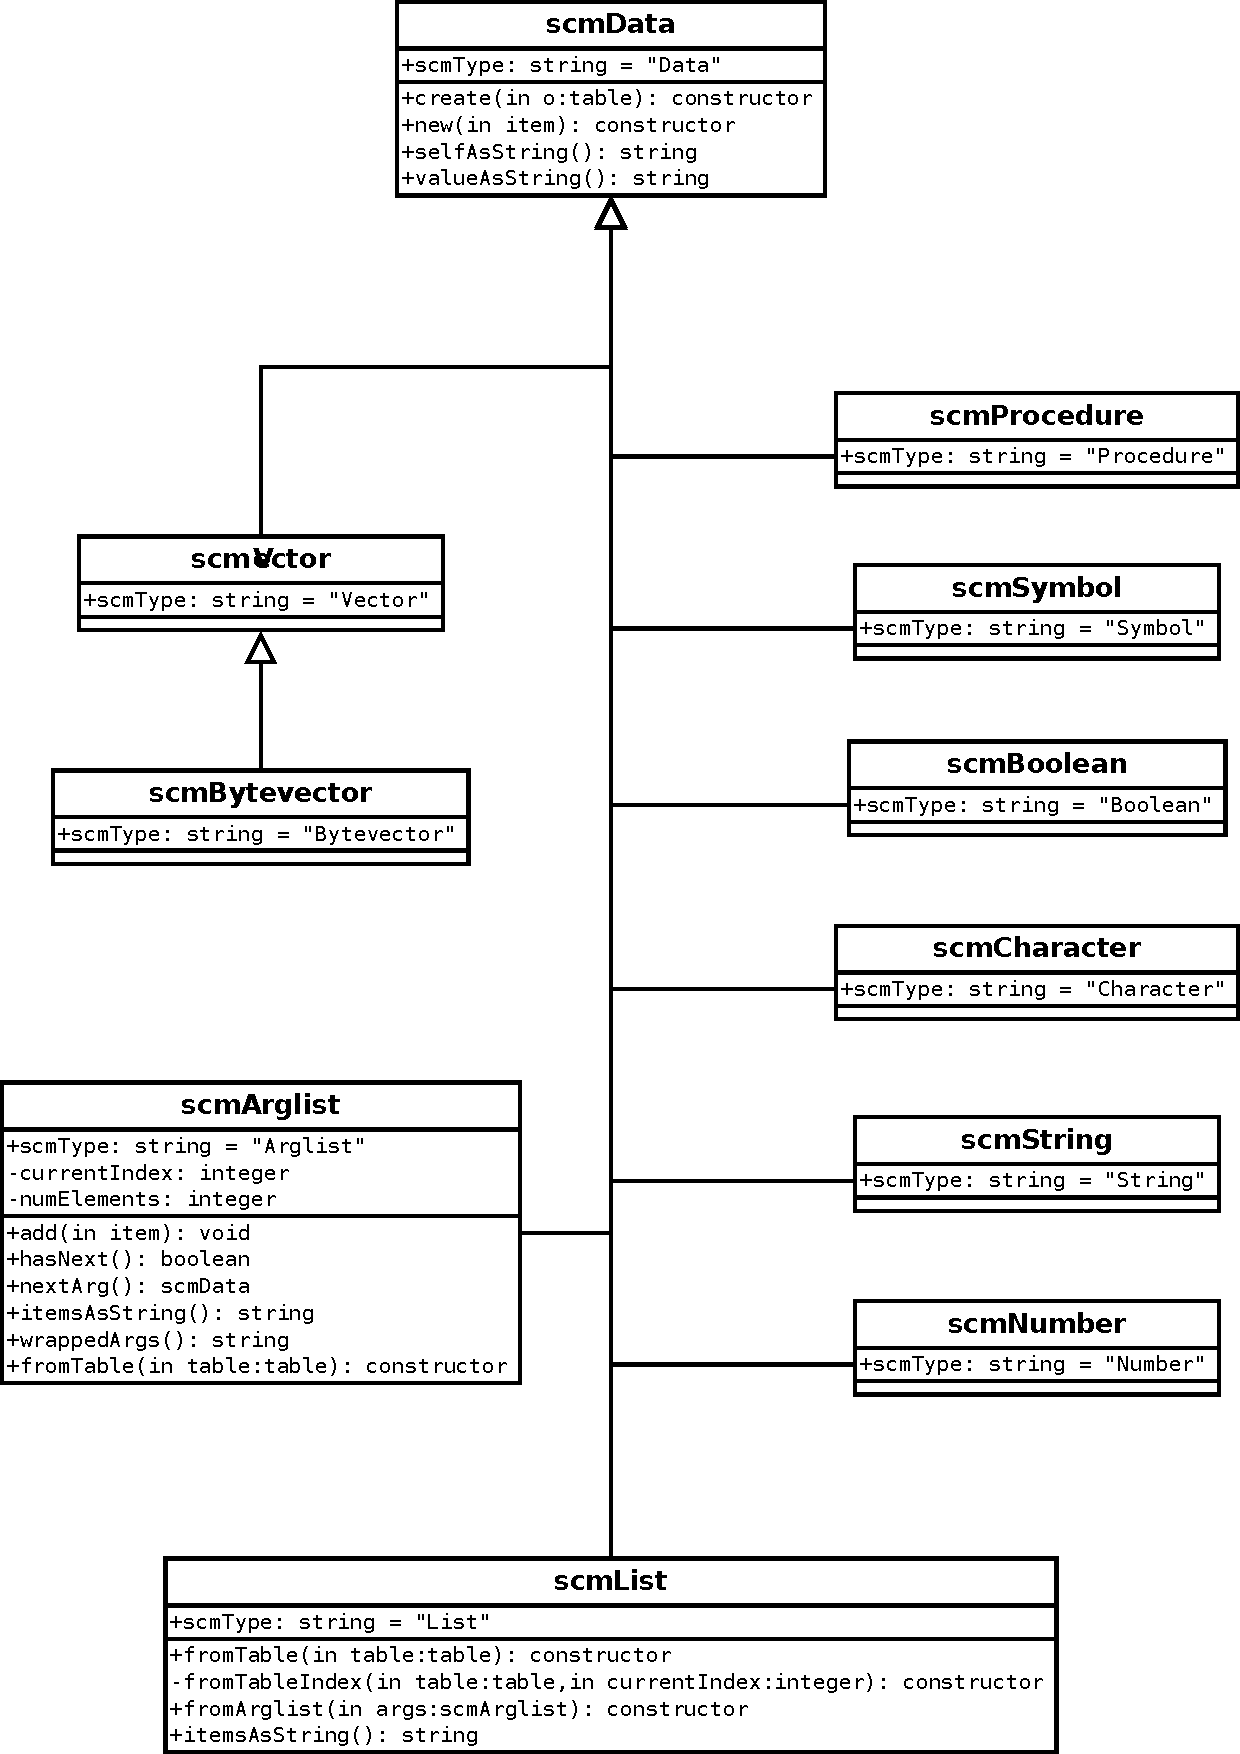
\includegraphics[width=\textwidth]{scmDataUML.pdf}
\caption{The structure of the intermediate data types}
\label{fig:scmDataUML}
\end{figure}

As can be seen in figure~\ref{fig:scmDataUML}


\section{The Operation Of A Translated Program}

The output of the translator consists of two main parts: a library of supported
Scheme functions and operations, written in Lua; and the translated output of
the the scheme input program, which uses the library to carry out its purpose.
All of the functions of the library deal with data in the intermediate form, as
output by the parser. That is to say that all function arguments and all of the
return values are in this form.

\end{comment} % TODO Remove this
\chapter{Testing}
Unit Tests were performed on the two main components of the translator, namely
the scanner and the parser. Once they were working properly, testing consisted
mainly of extending the functionality of the translator to correctly translate a
series of example Scheme programs.

\section{Unit Tests}


\section{Scheme Programs}


\section{Speed Tests}

\begin{table}
\centering
\begin{tabular}{|l|c|c|c|}
\hline
& lua & luaJIT & scm \\
\hline
First 1000 Primes & 0:16 & 0:09 & 0:02 \\ \hline
First 2000 Primes & 1:13 & 0:41 & 0:09 \\ \hline
First 5000 Primes & 8:26 & 4:49 & 1:02 \\ \hline
\end{tabular}
\caption{Test table}
\end{table}

\begin{table}
\centering
\begin{tabular}{|l|c|c|c|}
\hline
& lua & luaJIT & scm \\
\hline
Primes Up To 10000 & 0:37 & 0:16 & 0:03 \\ \hline
Primes Up To 20000 & FAIL & 1:13 & FAIL \\ \hline
\end{tabular}
\caption{Test table}
\end{table}

\begin{comment} % TODO Remove this

\chapter{Conclusion (5 pages)}
\section{Pitfalls}


\section{Further Work}

\subsection{Increasing Language Coverage}

\subsection{Features}

Continuations

Syntax Extension

File I/O

\section{A Final Word}

This project was intensely enjoyable and challenging, encapsulating a spectrum
of emotions from frustration to euphoria. It was an unrivaled opportunity for me
to let loose and have fun with computer languages, learning two new ones along
the way; but knowing how much this project means to Dr.\ Manning, I also felt a
responsibility to do it justice. If I had my time again I'd do some things
differently, and that is the measure of a great learning experience.

I would like to finish by acknowledging those who helped with the project:
\begin{itemize}
\item Thanks to my girlfriend, Shirley, and my mother, Mary, for proof-reading
and endless cups of Earl Grey.
\item Thanks to James Doherty and the System Administrators in the Computer
Science Department for the constant advice, backup and support throughout the
project. Fortunately I didn't have occasion to avail of it very often, but I
always knew it was there if I needed it.
\item Thanks to Professor Provan, and all the others who came to see my project
on open day.
\item And finally, many thanks to Dr.\ Manning, who provided inspiration,
guidance, great advice, and a truly fascinating project.
\end{itemize}



%
% Appendices
%

\appendix

\chapter{Program Source Code}
\section{Core}
\subsection{scheme2lua (Shell Script)}

\scriptsize

\begin{verbatim}
#!/bin/bash

cat dataTypes.lua
cat procedures.lua
for inputFile in $@; do
    LUA_PATH='?.lua;'${LUA_PATH} lua scheme2lua.lua < $inputFile
done
\end{verbatim}

\subsection{scheme2lua.lua}
\begin{verbatim}
require("parser")
require("procedures")
require("scanner")

-- Output the preamble
-- io.input("procedures.lua")
-- io.write(io.read("*a"))
io.input(io.stdin)

-- The main loop for the translator
scanner.init()
local expression = parser.parse(scanner.nextToken())
while expression ~= nil do
    print(tostring(expression))
    expression = parser.parse(scanner.nextToken())
end
\end{verbatim}

\subsection{scanner.lua}
\begin{verbatim}
module(..., package.seeall)

local stripLineComment, stripBlockComment, stripDatumComment
local charCache
local tokenCache

--
-- Return true if 'x' is a whitespace character
--
local function isWhiteSpace(x)
    return string.match(x, "^[%s]$")
end

--
-- Return true if 'x' is a delimiter
-- (For symbols, numbers, characters, booleans and the dotted pair marker)
--
local function isDelimiter(x)
    return isWhiteSpace(x) or x == ""
    or string.match(x, "^[%[%]%(%)\"';]$")
end

--
-- Return true if 'x' is a valid first character for a symbol
-- TODO Escaped Hex and Unicode characters currently not supported
--
local function isInitialSymbolChar(x)
    return string.match(x, "^[%a!&/:<=>~_%^%$%*%?%%]$")
end

--
-- Return true if 'x' is a valid subsequent character for a symbol
-- TODO Escaped Hex and Unicode characters currently not supported
--
local function isSubsequentSymbolChar(x)
    return isInitialSymbolChar(x) or string.match(x, "^[%d%.%+%-@]$")
end

--
-- Set up the scanner
--
function init()
    charCache = nil
    tokenCache = nil
end

--
-- Remove and return the next input character
--
local function nextChar()
    local result
    if charCache then
        result = charCache
        charCache = nil
    elseif not io.read(0) then
        result = ""
    else
        result = io.read(1)
    end
    return result
end

--
-- Return the next input character without removing it
--
local function peekChar()
    if not charCache then
        charCache = nextChar()
    end
    return charCache
end

--
-- Remove and return the next token from the scanner
--
function nextToken()
    local token
    local value = nil
    local c

    if tokenCache then
        token, value = tokenCache[1], tokenCache[2]
        tokenCache = nil
        return token, value
    end

    repeat
        c = nextChar()
        if c == ";" then
            c = stripLineComment()
        elseif c == "#" and peekChar() == "|" then
            c = stripBlockComment()
        elseif c == "#" and peekChar() == ";" then
            c = stripDatumComment()
        end
    until not isWhiteSpace(c) or c == ""

    if c == "" then
        token = "EOF"

    -- Check for peculiar symbols '+' and '-'
    elseif (c == "+" or c == "-") and isDelimiter(peekChar()) then
        token = c

    -- Check for peculiar symbol '...'
    elseif c == "." and peekChar() == "."
        and nextChar() == "." and peekChar == "." then
        nextChar()
        token = "..."

    elseif c == "-" and peekChar() == ">"   -- Another peculiar symbol
        or isInitialSymbolChar(c) then      -- Regular symbol
        local symbolValue = c
        while isSubsequentSymbolChar(peekChar()) do
            c = nextChar()
            symbolValue = symbolValue .. c
        end
        token, value = "Symbol", symbolValue

    elseif c == "#" and string.match(peekChar(), "[TtFf]") then
        token = "Boolean"
        if string.match(nextChar(), "[Tt]") then
            value = true
        else
            value = false
        end

    elseif c == "#" and peekChar() == "\\" then
        --
        -- TODO Named and hex characters currently not supported
        --
        token = "Character"
        nextChar()
        value = nextChar()
        
    elseif c == "\"" then
        --
        -- TODO Escape characters and multiline strings currently not
        -- supported
        --
        local stringValue = ""
        c = nextChar()
        while c ~= "\"" and c ~= "" do
            stringValue = stringValue .. c
            c = nextChar()
        end
        token, value = "String", stringValue

    elseif c == "#" and string.match(peekChar(), "[bodxie]")
        --
        -- TODO Numbers not properly supported yet
        --
        or string.match(c, "[+%-%d]") then
        local numberValue = string.byte(c) - string.byte("0")
        while string.match(peekChar(), "%d") do
            c = nextChar()
            local digit = string.byte(c) - string.byte("0")
            numberValue = 10 * numberValue + digit
        end
        token, value = "Number", numberValue
        
    elseif c == "#" and peekChar() == "(" then
        nextChar()
        token = "#("

    elseif c == "#" and string.match(peekChar(), "[vV]")
        and nextChar() and string.match(peekChar(), "[uU]") then
        nextChar()
        nextChar()
        token = "#vu8("

    else token = c
        --
        -- TODO Checking for invalid tokens currently not supported
        --
    end

    return token, value
end

--
-- Return the next token from the scanner without removing it
--
function peekToken()
    if tokenCache then
        return tokenCache[1], tokenCache[2]
    else
        local token, value = nextToken()
        tokenCache = {token, value}
        return token, value
    end
end

--
-- Remove a line comment from the scanner and return the next character
--
stripLineComment = function ()
    local c
    repeat
        c = nextChar()
    until c == "\n" or c == ""
    return c
end

--
-- Remove a block comment from the scanner and return the next character
--
stripBlockComment = function ()
    local c
    local nestLevel = 1
    nextChar()
    repeat
        c = nextChar()
        if c == "#" and nextChar() == "|" then
            c = nextChar()
            nestLevel = nestLevel + 1
        elseif c == "|" and nextChar() == "#" then
            c = nextChar()
            nestLevel = nestLevel - 1
        end
    until nestLevel == 0 or c == ""
    return c
end

--
-- Remove a block comment from the scanner and return the next character
-- TODO Datum comments not currently supported
--
stripDatumComment = function ()
    return c
end
\end{verbatim}

\subsection{parser.lua}
\begin{verbatim}
module(..., package.seeall)

require("dataTypes")
require("forms")
require("scanner")

local applyFunction, getArguments, readCompound

--
-- Return an iterator over the arguments in a Scheme list syntactic form
--
getArguments = function ()
    return function ()
        local token, value = scanner.peekToken()
        if token == ")" or token == "]" then
            return nil
        end
        return scanner.nextToken()
    end
end

--
-- Return the set of Scheme function arguments from the scanner as a
-- string
--
gatherArguments = function (funcName)
    if forms.specialArgs[funcName] then
        return forms.specialArgs[funcName]()
    else
        local result = scmArglist:new()
        for arg, argValue in getArguments() do
            result:add(parse(arg, argValue))
        end
        if forms.wrappedArgs[funcName] then
            return result:wrappedArgs()
        end
        return result:selfAsString()
    end
end

--
-- Apply the Scheme function 'func'
--
applyFunction = function (func)
    local f = tostring(func)
    if forms.specialSyntax[f] then
        return forms.specialSyntax[f]()
    end
    return (forms.procedures[f] or f)
    .. "(" .. gatherArguments(f) .. ")"
end

--
-- Read and return a single scheme datum from the scanner
--
readDatum = function ()
    local token, value = scanner.peekToken()
    if token == "(" or token == "[" then
        scanner.nextToken()   -- Remove initial bracket
        local list = readList()
        scanner.nextToken()   -- Remove ending bracket
        return list
    elseif token == "#(" or token == "#vu8(" then
        return readVector()
    end
    scanner.nextToken()
    return parse(token, value)
end

--
-- Read and return a scheme list from the scanner (not including brackets)
--
readList = function ()
    local token = scanner.peekToken()
    if token == ")" or token == "]" then
        return scmList:new()
    elseif token == "." then
        scanner.nextToken()
        return readDatum()
    else
        return scmList:new{car = readDatum(); cdr = readList()}
    end
end

--
-- Read and return a scheme vector or bytevector from the scanner (including
-- brackets)
--
readVector = function ()
    local token = scanner.nextToken()
    local objectType = scmVector
    local value = {}
    if token == "#vu8(" then
        objectType = scmBytevector
    end
    token = scanner.peekToken()
    while token ~= ")" do
        table.insert(scmValue, readDatum())
        token = scanner.peekToken()
    end
    scanner.nextToken()
    return objectType:new(value)
end

--
-- Evaluate the Scheme token 'token', with value 'value', and return an scmData
-- encapsulating the appropriate Lua translation
--
function parse(token, value)
    if token == "EOF" then
        return nil
    end

    if token == "Boolean" then
        return scmBoolean:new(value)

    elseif token == "Character" then
        return scmCharacter:new(value)

    elseif token == "String" then
        return scmString:new(value)

    elseif token == "Number" then
        return scmNumber:new(value)

    elseif token == "Symbol" then
        return scmSymbol:new(value)

    elseif token == "(" or token == "[" then
        local procedureValue = applyFunction(parse(scanner.nextToken()))
        scanner.nextToken()
        return scmProcedure:new(procedureValue)

    elseif token == "'" then
        return readDatum()

    else
        return scmData:new(token)
    end
end
\end{verbatim}

\subsection{forms.lua}
\begin{verbatim}
module(..., package.seeall)

require("parser")
require("scanner")

--
-- A utility function that returns the string representation of a sequence of
-- scheme expressions (or "body"s) from the scanner, returning the last one.
-- This is a common syntax for lambda, case-lambda, cond, let and others
--
local function bodyList()
    local result = ""
    local token = scanner.peekToken()
    while token ~= ")" do
        local expr = parser.parse(scanner.nextToken())
        if scanner.peekToken() == ")" then
            result = result .. "return "
        end
        result = result .. expr:selfAsString() .. "\n"
        token = scanner.peekToken()
    end
    return result
end;

--
-- A table of supported special syntaxes. Each is a function that returns the
-- final output string for that syntax.
--
specialSyntax = {
    ["cond"] = function ()
        local result = "(function ()\n"
            local token = scanner.peekToken()
            local first = true
            while token ~= ")" do
                scanner.nextToken()  -- Remove initial bracket of clause
                local test = parser.parse(scanner.nextToken())
                if first then
                    result = result .. "if "
                    .. test:selfAsString() .. ".value then\n"
                    first = false
                elseif tostring(test) == "else" then
                    result = result .. "else\n"
                else
                    result = result .. "elseif "
                    .. test:selfAsString() .. ".value then\n"
                end
                local expr = scanner.peekToken()
                if expr == "=>" then
                    scanner.nextToken()
                    local func = parser.parse(scanner.nextToken())
                    result = result .. "return " .. func:selfAsString() ..
                    "(" .. test:selfAsString() .. ")\n"
                elseif expr == ")" then
                    scanner.nextToken()
                    result = result .. "return " .. test:selfAsString() .. "\n"
                else
                    result = result .. bodyList()
                    scanner.nextToken()
                end
                token = scanner.peekToken()
            end
            return result .. "end end)()\n"
        end;

    ["define"] = function ()
        -- TODO implement other forms of define
        local assignee = parser.parse(scanner.nextToken())
        local object = parser.parse(scanner.nextToken())
        return assignee:selfAsString() .. " = " .. object:selfAsString()
    end;

    ["if"] = function ()
        local result = "(function ()\nif "
            .. parser.parse(scanner.nextToken()):selfAsString()
            .. ".value then\nreturn"
            .. parser.parse(scanner.nextToken()):selfAsString() .. "\n"
        if scanner.peekToken() ~= ")" then
            result = result .. "else\nreturn"
            .. parser.parse(scanner.nextToken()):selfAsString() .. "\n"
        end
        return result .. "end end)()\n"
    end;

    ["lambda"] = function ()
        local paramList = {}
        local vararg = false
        local params = parser.readDatum()
        if params.scmType == "List" then
            while params.value ~= nil do
                table.insert(paramList, scmSymbol:new(params.value.car))
                if params.value.cdr.scmType ~= "List" then
                    vararg = params.value.cdr
                    break
                end
                params = params.value.cdr
            end
        else
            vararg = params
        end
        local result = "(function ("
            .. scmArglist.fromTable(paramList):selfAsString()
            .. (vararg and "..." or "") .. ")\n"
            if vararg ~= false then
                result = result .. "local " .. tostring(vararg)
                .. " = scmList.fromTable{...}\n"
            end
            result = result .. bodyList() .. "end)"
        return result
    end;

    ["let"] = function ()
        local funcName = nil
        if scanner.peekToken() == "Symbol" then
            funcName = tostring(parser.parse(scanner.nextToken()))
        end
        scanner.nextToken() -- Opening '(' of var list
        local varNames = {}
        local varValues = {}
        local token = scanner.peekToken()
        while token ~= ")" do
            scanner.nextToken() -- Opening '(' of var definition
            table.insert(varNames, parser.parse(scanner.nextToken()))
            table.insert(varValues, parser.parse(scanner.nextToken()))
            scanner.nextToken() -- Closing ')' of var definition
            token = scanner.peekToken()
        end
        scanner.nextToken() -- Closing ')' of var list
        local funcDef = "(function "
            .. "(" .. scmArglist.fromTable(varNames):selfAsString() .. ")\n"
            .. bodyList() .. "end)"
        local args = scmArglist.fromTable(varValues):selfAsString()
        if funcName then
            return "(function ()\n" .. funcName .. " = " .. funcDef
                .. "\nreturn " .. funcName .. "(" .. args .. ") end)()\n"
        else
            return funcDef .. "(" .. args .. ")\n"
        end
    end;
}

--
-- A table for scheme functions that need all of their arguments wrapped in
-- functions. This prevents the arguments from being fully evaluated and is
-- useful for short-circuit operations
--
wrappedArgs = {
    ["and"] = true;
    ["or"] = true;
}

--
-- A table for scheme functions that need their arguments collected in a
-- non-standard way. Each is a function that returns the argument list as a
-- string.
--
specialArgs = {
    ["quote"] = function ()
        return parser.readDatum():selfAsString()
    end;
}

--
-- A table of the supported Scheme procedures
--
procedures = {
    ["cond"] = "s2l_cond";
    ["quote"] = "s2l_quote";

    ["cons"] = "s2l_cons";
    ["car"] = "s2l_car";
    ["cdr"] = "s2l_cdr";
    ["list"] = "s2l_list";
    ["length"] = "s2l_length";
    ["filter"] = "s2l_filter";

    -- Useful output routines
    ["display"] = "s2l_display";
    ["newline"] = "s2l_newline";

    -- Arithmetic operators
    ["+"] = "s2l_arithmeticPlus";
    ["-"] = "s2l_arithmeticMinus";
    ["*"] = "s2l_arithmeticMultiply";
    ["/"] = "s2l_arithmeticDivide";

    -- Relational operators
    ["<"] = "s2l_lessThan";
    ["<="] = "s2l_lessThanOrEqual";
    ["="] = "s2l_equals";
    [">"] = "s2l_greaterThan";
    [">="] = "s2l_greaterThanOrEqual";
    ["eqv?"] = "s2l_equals";   -- FIXME

    -- Boolean operators
    ["and"] = "s2l_and";
    ["or"] = "s2l_or";
    ["not"] = "s2l_not";

    -- Predicates
    ["pair?"] = "s2l_pair";
    ["boolean?"] = "s2l_boolean";
    ["null?"] = "s2l_null";
    ["number?"] = "s2l_number";
    ["integer?"] = "s2l_integer";

    -- Exit
    ["exit"] = "s2l_exit";
    ["quit"] = "s2l_exit";
}
\end{verbatim}

\subsection{dataTypes.lua}
\begin{verbatim}
--
-- SCHEME TO LUA TRANSLATOR
-- Preamble File 1
-- This file contains lua container tables for scheme data
--

--
-- Container for basic scheme data. Actual types inherit from this.
-- Noteworthy methods:
-- selfAsString - an (overrideable) object function that returns a string of
-- lua code that will recreate that object
-- valueAsString - an (overrideable) object function that returns the output
-- representation of that scheme object
--
scmData = {
    scmType = "Data";
    create = function (self, o)
        local result = o or {}
        setmetatable(result, self)
        self.__index = self
        self.__tostring = self.valueAsString or scmData.valueAsString
        return result
    end;
    new = function (self, item)
        return self:create{value = item}
    end;
    selfAsString = function (self)
        local funcName = "scm" .. self.scmType .. ":new"
        return funcName .. "("..tostring(self.value)..")"
    end;
    valueAsString = function (self)
        return tostring(self.value)
    end;
}

--
-- This wraps scheme function arguments with an iterative interface
--
scmArglist = scmData:create{
    scmType = "Arglist";
    currentIndex = 1;
    numElements = 0;
    add = function (self, item)
        if self.value == nil then
            self.value = {}
        end
        self.numElements = self.numElements + 1
        self.value[self.numElements] = item
    end;
    hasNext = function (self)
        return self.currentIndex > self.numElements
    end;
    nextArg = function (self)
        local result = self.value[self.currentIndex]
        self.currentIndex = self.currentIndex + 1
        return result
    end;
    itemsAsString = function (self)
        local result = ""
        for _, item in ipairs(self.value) do
            result = result .. item:selfAsString() .. ", "
        end
        if result ~= "" then
            result = string.sub(result, 1, -3)
        end
        return result
    end;
    selfAsString = function (self)
        if self.numElements == 0 then
            return ""
        end
        return self:itemsAsString()
    end;
    wrappedArgs = function (self)
        if self.numElements == 0 then
            return ""
        end
        local result = ""
        for _, item in ipairs(self.value) do
            result = result .. "(function () return " .. item:selfAsString()
                .. " end), "
        end
        if result ~= "" then
            result = string.sub(result, 1, -3)
        end
        return result
    end;
    fromTable = function (table)
        local result = scmArglist:new()
        for _, value in ipairs(table) do
            result:add(value)
        end
        return result
    end;
}

--
-- Data type to hold a scheme procedure
--
scmProcedure = scmData:create{
    scmType = "Procedure";
    selfAsString = function (self)
        return tostring(self.value);
    end;
}

--
-- Data type to hold a scheme symbol
--
scmSymbol = scmData:create{
    scmType = "Symbol";
    selfAsString = function (self)
        return self:valueAsString();
    end;
}

--
-- Data type to hold a scheme boolean
--
scmBoolean = scmData:create{
    scmType = "Boolean";
    valueAsString = function (self)
        return "#" .. (self.value and "t" or "f")
    end;
}

--
-- Data type to hold a scheme character
--
scmCharacter = scmData:create{
    scmType = "Character";
    selfAsString = function (self)
        return "scmCharacter:new(\"" .. self.value .. "\")"
    end;
}

--
-- Data type to hold a scheme string
--
scmString = scmData:create{
    scmType = "String";
    selfAsString = function (self)
        return "scmString:new(\"" .. self.value .. "\")"
    end;
}

--
-- Data type to hold a scheme number
--
scmNumber = scmData:create{
    scmType = "Number";
}

--
-- Data type to hold a scheme list
--
scmList = scmData:create{
    scmType = "List";
    fromTable = function (table)
        return scmList.fromTableIndex(table, 1)
    end;
    fromTableIndex = function (table, currentIndex)
        if table[currentIndex] == nil then
            return scmList:new()
        elseif tostring(table[currentIndex]) == "." then
            return table[currentIndex + 1]
        else
            return scmList:new{
                car = table[currentIndex];
                cdr = scmList.fromTableIndex(table, currentIndex + 1)
            }
        end
    end;
    fromArglist = function (args)
        return scmList.fromTableIndex(args.value, args.currentIndex)
    end;
    itemsAsString = function (self)
        if self.value == nil then
            return ""
        end
        local car = self.value.car
        local cdr = self.value.cdr
        if cdr.scmType ~= "List" then
            return tostring(car) .. " . " .. tostring(cdr)
        elseif cdr.value == nil then
            return tostring(car)
        else
            return tostring(car) .. " " .. cdr:itemsAsString()
        end
    end;
    selfAsString = function (self)
        if self.value == nil then
            return "scmList:new()"
        end
        return "scmList:new{\ncar = " .. self.value.car:selfAsString()
        .. ";\ncdr = " .. self.value.cdr:selfAsString() .. "}"
    end;
    valueAsString = function (self)
        return "(" .. self:itemsAsString() .. ")"
    end;
}

--
-- Data type to hold a scheme vector
--
scmVector = scmData:create{
    scmType = "Vector";
    itemsAsString = function (self)
        local result = ""
        for _, v in ipairs(self.value) do
            result = result .. tostring(v) .. " "
        end
        if result ~= "" then
            result = string.sub(result, 1, -2)
        end
        return result
    end;
    valueAsString = function (self)
        return "#(" .. self:itemsAsString() .. ")"
    end;
}

--
-- Data type to hold a scheme bytevector
--
scmBytevector = scmVector:create{
    scmType = "Bytevector";
    valueAsString = function (self)
        return "#vu8(" .. self:itemsAsString() .. ")"
    end;
}
\end{verbatim}

\subsection{procedures.lua}
\begin{verbatim}
--
-- SCHEME TO LUA TRANSLATOR
-- Preamble File 2
-- This file contains the lua implementation of the scheme functions
--

--
-- BEGIN SCHEME FUNCTIONS
--

function s2l_quote(obj)
    return obj
end

function s2l_cons(obj1, obj2)
    return scmList:new{car = obj1; cdr = obj2}
end

function s2l_car(pair)
    return pair.value.car
end

function s2l_cdr(pair)
    return pair.value.cdr
end

function s2l_list(...)
    return scmList.fromTable{...}
end

function s2l_length(list)
    local result = 0
    while not s2l_null(list).value do -- FIXME Clean up (metamethods maybe)
        result = result + 1
        list = s2l_cdr(list)
    end
    return scmNumber:new(result)
end

function s2l_filter(proc, list)
    if s2l_null(list).value then -- FIXME Clean up (metamethods maybe)
        return scmList:new()
    elseif proc(s2l_car(list)).value then -- FIXME Clean up (metamethods maybe)
        return s2l_cons(s2l_car(list), s2l_filter(proc, s2l_cdr(list)))
    else
        return s2l_filter(proc, s2l_cdr(list))
    end
end

function s2l_display(obj)
    io.write(tostring(obj))
end

function s2l_newline()
    io.write("\n")
end

function s2l_arithmeticPlus(...)
    local result = 0
    for _, item in ipairs{...} do
        result = result + item.value
    end
    return scmNumber:new(result)
end

-- FIXME
function s2l_arithmeticMinus(a, b)
    return scmNumber:new(a.value - b.value)
end

function s2l_arithmeticMultiply(...)
    local result = 1
    for _, item in ipairs{...} do
        result = result * item.value
    end
    return scmNumber:new(result)
end

-- FIXME
function s2l_arithmeticDivide(a, b)
    return scmNumber:new(a.value / b.value)
end

function s2l_lessThan(n1, n2)
    return scmBoolean:new(n1.value < n2.value)
end

function s2l_lessThanOrEqual(n1, n2)
    return scmBoolean:new(n1.value <= n2.value)
end

function s2l_equals(n1, n2)
    return scmBoolean:new(n1.value == n2.value)
end

function s2l_greaterThan(n1, n2)
    return scmBoolean:new(n1.value > n2.value)
end

function s2l_greaterThanOrEqual(n1, n2)
    return scmBoolean:new(n1.value >= n2.value)
end

-- Short circuit
function s2l_and(...)
    local result = scmBoolean:new(true)
    for _, f in ipairs{...} do
        local item = f()
        if item.value == false then
            return scmBoolean:new(false)
        else
            result = item
        end
    end
    return result
end

-- Short circuit
function s2l_or(...)
    for _, f in ipairs{...} do
        local item = f()
        if item.value then
            return item
        end
    end
    return scmBoolean:new(false)
end

function s2l_not(obj)
    if obj.value == false then
        return scmBoolean:new(true)
    end
    return scmBoolean:new(false)
end

function s2l_pair(obj)
    return scmBoolean:new(obj.scmType == "List" and obj.value ~= nil)
end

function s2l_boolean(obj)
    return scmBoolean:new(obj.scmType == "Boolean")
end

function s2l_null(obj)
    return scmBoolean:new(obj.scmType == "List" and obj.value == nil)
end

function s2l_number(obj)
    return scmBoolean:new(obj.scmType == "Number")
end

function s2l_integer(obj)
    return scmBoolean:new(obj.scmType == "Number" and obj.value % 1 == 0)
end

function s2l_exit()
    return nil
end

--
-- END SCHEME FUNCTIONS
--
\end{verbatim}


\section{Unit Tests}
\subsection{run-tests (Shell Script)}
\begin{verbatim}
#!/bin/bash

for testsuite in tests/*.lua; do
    LUA_PATH='?.lua;tests/?.lua;'${LUA_PATH} lua $testsuite
done
\end{verbatim}

\subsection{scannertest.lua}
\begin{verbatim}
require("scanner")

--
-- Create test input file
--
io.output("/tmp/s2ltest_chars.scm")
io.write("(+ 1 2)\n")
io.write("(display \"abc\")\n")
io.close()

io.output("/tmp/s2ltest_tokens.scm")
io.write("(newline) ; This should print a newline\n")
io.write("#| Commented out section\n")
io.write("(+ 1 2)\n")
io.write("(define x #| Nested #| Another nest |# block comment |# 5)\n")
io.write("(display \"abc\")\n")
io.write("End of commented out section |#\n")
io.write("; Another one-line comment|#\n")
io.write("(lambda (->x) (+ ->x 1))\n")
io.write("(* (+ 3 5) 2 3)\n")
io.close()

io.output(io.stdout)

characters = {
    "(", "+", " ", "1", " ", "2", ")", "\n",
    "(", "d", "i", "s", "p", "l", "a", "y", " ",
    "\"", "a", "b", "c", "\"", ")", "\n", 
}

tokens = {
    {"("}, {"symbol", "newline"}, {")"},
    {"("}, {"symbol", "lambda"},
	{"("}, {"symbol", "->x"}, {")"},
	{"("}, {"+"}, {"symbol", "->x"}, {"number", 1}, {")"},
    {")"},
    {"("}, {"symbol", "*"},
	{"("}, {"+"}, {"number", 3}, {"number", 5}, {")"},
	{"number", 2}, {"number", 3},
    {")"}
}

--
-- Run tests
--

-- Test char functions
io.input("/tmp/s2ltest_chars.scm")
scanner.init()
local index = 1
while scanner.peekChar() ~= "" do
    assert(scanner.peekChar() == characters[index]
    and scanner.nextChar() == characters[index])
    index = index + 1
end

-- Test token functions
io.input("/tmp/s2ltest_tokens.scm")
scanner.init()
index = 1
while scanner.peekToken() ~= "EOF" do
    local token, value = scanner.peekToken()
    assert(token == tokens[index][1] and value == tokens[index][2])
    token, value = scanner.nextToken()
    assert(token == tokens[index][1] and value == tokens[index][2])
    index = index + 1
end

print("Scannertest: All tests passed")
\end{verbatim}

\subsection{parsertest.lua}
\begin{verbatim}
require("parser")
require("scanner")

--
-- Create test input file
--
io.output("/tmp/s2ltest_parser.scm")
io.write("display \"abc\"\n")
io.write("123 #\\l\n")
io.write("#f #t")
io.write("5 (\"a\" (1 2 3) #t #\\m)")
io.close()

io.output(io.stdout)

--
-- Run tests
--
io.input("/tmp/s2ltest_parser.scm")
scanner.init()
if assert(parser.evaluate(scanner.peekToken()) == "display") 
    and assert(parser.evaluate(scanner.nextToken()) == "display") 
    and assert(parser.evaluate(scanner.nextToken()) == "\"abc\"") 
    and assert(parser.evaluate(scanner.nextToken()) == 123) 
    and assert(parser.evaluate(scanner.nextToken()) == "\"l\"") 
    and assert(parser.evaluate(scanner.nextToken()) == false) 
    and assert(parser.evaluate(scanner.nextToken()) == true) 
    and assert(parser.readDatum() == 5) 
    and assert(parser.readDatum()[2][3] == 3) 
    then
    print("Parsertest: All tests passed")
end
\end{verbatim}

\normalsize


\chapter{Open Day Materials}
Test

\end{comment} % TODO Remove this

%
% References
%

\begin{thebibliography}{99}

  \bibitem{schemebook}
  \emph{Scheme and the Art of Programming} \\
  George Springer and Daniel P.\ Friedman,
  The MIT Press. \\
  ISBN 0-262-19288-8 \\
  Cited on the following pages: 

  \bibitem{tspl}
  \emph{The Scheme Programming Language} \\
  R.\ Kent Dybvig,
  Fourth Edition,
  The MIT Press. \\
  This online version was used: \url{http://www.scheme.com/tspl4/} \\
  ISBN 0-262-19288-8 \\
  Cited on the following pages: 

  \bibitem{r6rs}
  \emph{Revised $^6$ Report On The Algorithmic Language Scheme: Summary} \\
  Michael Sperber, R.\ Kent Dybvig, Matthew Flatt and Anton van Straaten, \\
  \url{http://www.r6rs.org/final/html/r6rs/r6rs-Z-H-1.html} \\
  Cited on the following pages: 

  \bibitem{luabook}
  \emph{Programming in Lua} \\
  Roberto Ierusalimschy,
  PUC-Rio, Brazil,
  2nd Edition,
  2006. \\
  ISBN 85-903798-2-5 \\
  Cited on the following pages: 
  
  \bibitem{luamanual}
  \emph{Lua 5.1 Reference Manual} \\
  Roberto Ierusalimschy, Luiz Henrique de Figueiredo and Waldemar Celes,
  PUC-Rio, Brazil,
  2006. \\
  This online version was used: \url{http://www.lua.org/manual/5.1/} \\
  ISBN 85-903798-3-3 \\
  Cited on the following pages: 
  
  \bibitem{evolua}
  \emph{The Evolution of Lua} \\
  Roberto Ierusalimschy, Luiz Henrique de Figueiredo and Waldemar Celes,
  PUC-Rio, Brazil. \\
  \url{http://www.tecgraf.puc-rio.br/~lhf/ftp/doc/hopl.pdf} \\
  Cited on the following pages: 
  
  \bibitem{luaslides}
  \emph{Small is Beautiful: the design of Lua} \\
  Lecture given at Stanford University \\
  Roberto Ierusalimschy,
  PUC-Rio, Brazil. \\
  Lecture slides: \\
  \url{http://www.stanford.edu/class/ee380/Abstracts/100310-slides.pdf} \\
  Cited on the following pages: 

  \bibitem{luajit}
  \emph{LuaJIT: Just-In-Time Compiler For Lua} \\
  Mike Pall. \\
  \url{http://luajit.org/} \\
  Cited on the following pages:

  \bibitem{compiler}
  \emph{Introduction To Compiler Construction With UNIX} \\
  Axel T.\ Schreiner and H.\ George Friedman Jr.,
  Prentice Hall,
  1985. \\
  This online version was used: \\
  \url{https://ritdml.rit.edu/bitstream/handle/%
       1850/8122/ASchreinerBook1985.pdf?sequence=1} \\
  ISBN: 978-0134743967
  Cited on the following pages:

  \bibitem{lualisp}
  \emph{Embedded Lisp -- via Lua} \\
  David Bergman (davber). \\
  \url{http://blog.davber.com/2006/09/07/embedded-lisp-via-lua/} \\
  Cited on the following pages: 
  
  \bibitem{sal}
  \emph{The Simple Applicative Language (SAL) Interpreter} \\
  Dr.\ Joseph Manning,
  Department Of Computer Science,
  University College Cork. \\
  Cited on the following pages: 

\end{thebibliography}



\end{document}
